% !TEX root =  ../master.tex
\chapter{Implementierung}

\section{Schnittstellen}
Die Simulation nutzt verschiedene Schnittstellen und bietet selbst auch einige an. Besonders durch die Aufteilung der Simulation in Frontend- und Backend-Server sind Schnittstellen notwendig.
Das Frontend nutzt dabei die Schnittstellen anderer Teams (vgl. \autoref{sec:otherTeams}) und des Backend-Servers.

Die Schnittstellen der Börse sind in \href{https://boerse.moonstonks.space/docs/}{https://boerse.moonstonks.space/docs/} und die Schnittstellen der Simulation in \href{https://simulation.moonstonks.space/docs/}{https://simulation.moonstonks.space/docs/} dokumentiert.

Die Simulation bietet dabei besonders die drei nachfolgenden Schnittstellen an:
\begin{itemize}
    \item Verfügbare Szenarios\\
        Gibt alle verfügbaren Szenarios zurück. Jedes Szenario gibt den Namen und die einzelnen Datenpunkte zurück, die bezogen auf die Uhrzeit die Kursveränderungen definieren.
    \item Szenario starten\\
        Diese Schnittstelle kann genutzt werden um ein Szenario zu starten.
    \item Szenario Status abfragen\\
        Diese Schnittstelle diehnt zur Abfrage, wie weit fortgeschritte ein Szenario ist. Hierbei wird ein Prozent-Wert zurückgegeben, der die simulierte Zeit repräsentiert. Sollte kein Szenario im Gange sein, gibt diese 100 zurück.
    \item Szenario stoppen\\
        Mit dieser Schnittstelle kann ein Szenario gestoppt werden. Die Simulation unterbricht alle ihre Orders und geht in einen Leerlauf.
\end{itemize}

% TODO: Das hier vielleicht in ein eigenes CI Kapitel verschieben?
Interne Schnittstellen und Funktionalitäten werden auserdem getestet.
Dafür ist eine Pipeline definiert, welche bei jeder Anpassung des Quellcodes diesen auf Fehler überprüft.
Die Ergebnisse werden anschlißend unter \href{https://stonks2moon.github.io/Simulation/coverage/}{https://stonks2moon.github.io/Simulation/coverage/} publiziert.

\section{Architektur}\label{sec:Architektur}
\begin{figure}[ht]
    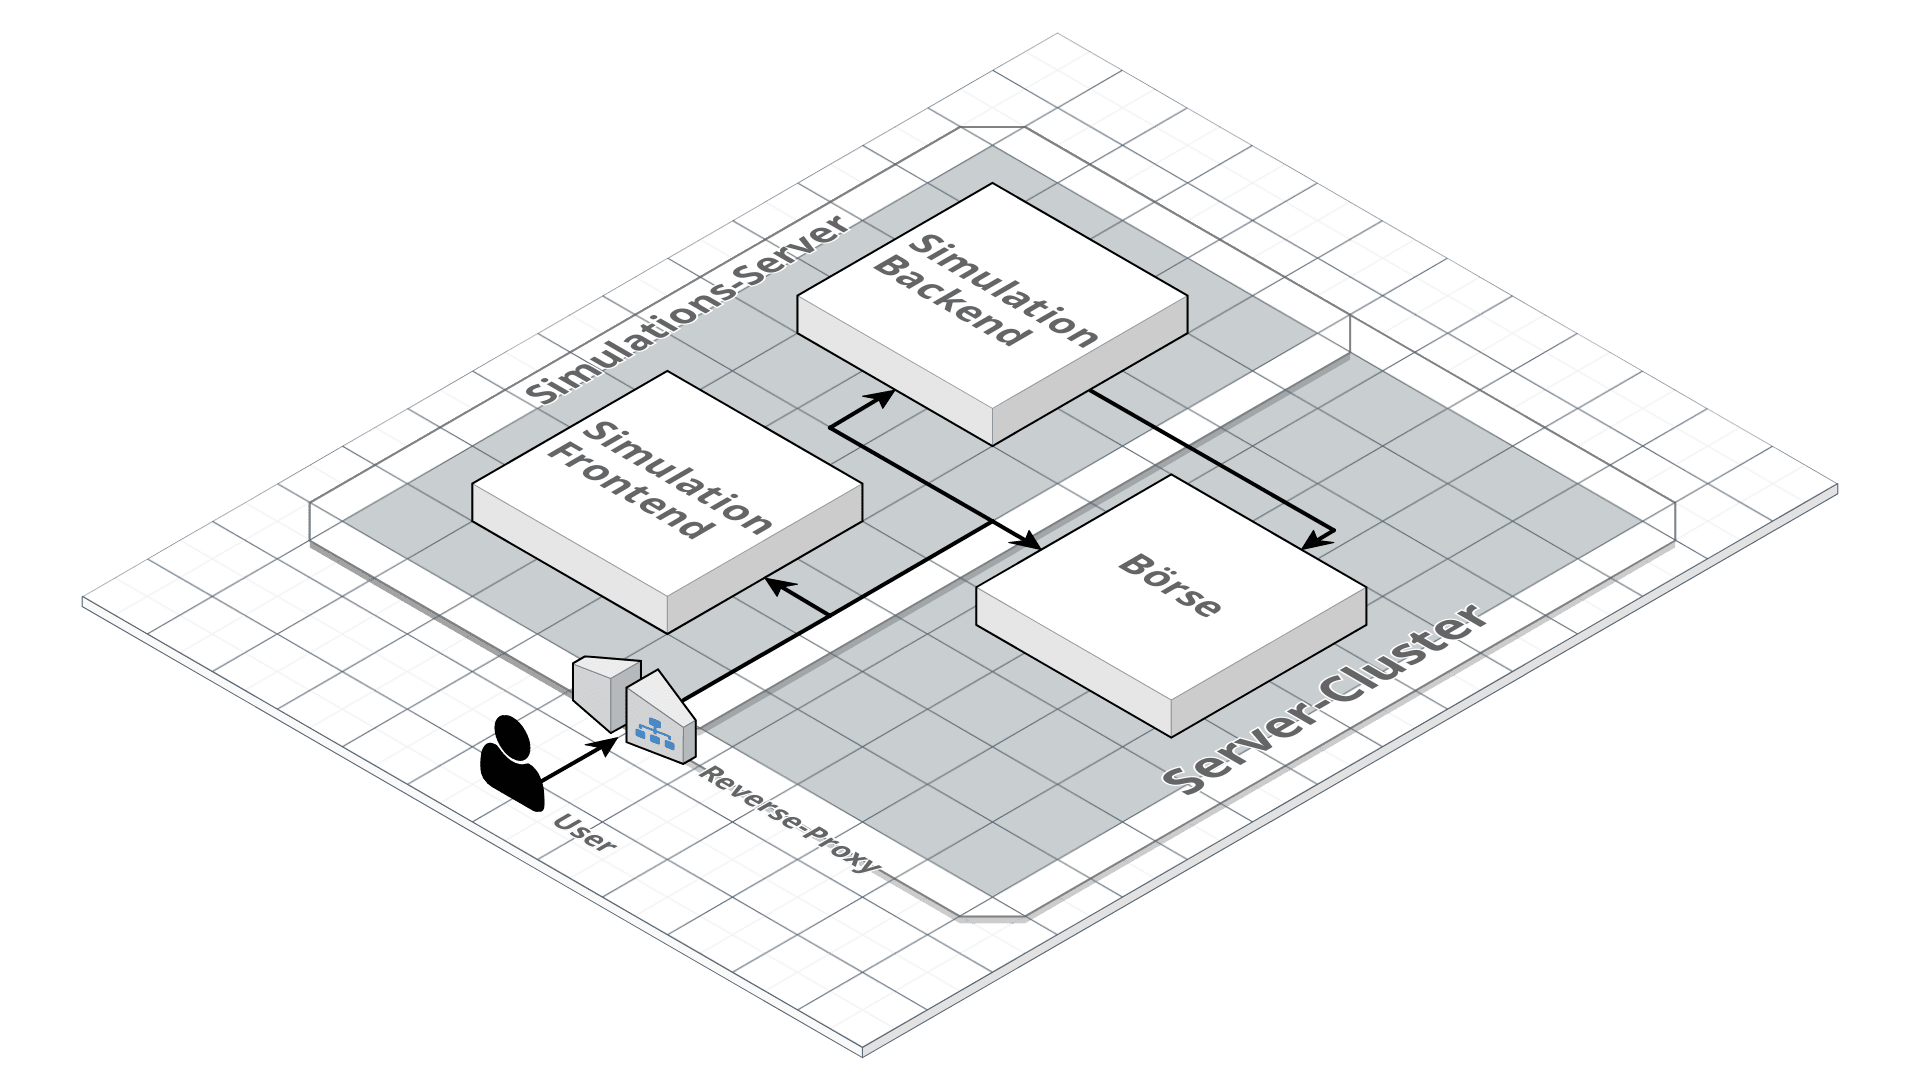
\includegraphics[width=\textwidth]{img/architecture.png}
    \centering
    \caption{Architektur}
    \label{fig:architecture}
\end{figure}

In \autoref{fig:architecture} ist die Architektur der Anwendung dargestellt.
Alle benötigten Server sind in einem Server-Cluster organisiert.
Hier werden die Börse, die Kernlogik der Simulation ausgeführt und das Nutzerinterface an den User ausgeliefert. Zentralles Eintrittstor ist dabei ein Reverse-Proxy, welcher die Aufgabe hat, die Daten an die richtigen internen Server weiterzuleiten und Daten, die für den Nutzer sind zu verschlüsseln.
Innerhalb des Clusters kommunizieren der Simulations-Backend-Server direkt mit der Börse. Dadurch kann dieser Verkehr nicht von außen beeinflusst werden und mögliche Aktieninformationen (beispielsweise welche Person welche Aktie handelt) sind geschützt.

Das Simulations-Frontend dient als grafische Benutzeroberfläche, mit dem das eigentliche Simulations-Backend gesteuert wird. Weitere Informationen dazu finden sich in \autoref{cha:Nutzerhandbuch}.

Unsere Architektur trennt dabei streng die Szenario-Logik vom Nutzerinterface.
Hat der Nutzer ein Szenario ausgewählt, alle Einstellungen getroffen und das Szenario gestartet, wird eine Anfrage an den Simulations-Backend-Server gesendet. Darauf hin beginnt dieser das entsprechende Szenario auszuführen und mit der Börse zu handeln.
Dies hat ein paar Vorteile gegenüber der Implementierung sämtlicher Logik innerhalb des Nutzerinterfaces:
\begin{enumerate}
    \item Zentrale Nutzersteuerung\\
        Der Backend-Server kann Ausführungen von Szenarien steuern. So werden beispielsweise Kollisionen vermieden, wenn mehrere Szenarien von verschiedenen Nutzern gestartet werden würden.
    \item Code-Qualität\\
        Durch die Trennung der Logik nach dem Separation-of-Concern und Clean-Code Methodiken wird der Quelltext wartbarer.
    \item Unterbrechungen\\
        Der Nutzer kann ein Szenario starten, welches eine längere Dauer hat (z.\,B. mehrere Tage). Anschließend muss er nicht seinen COmputer eingeschaltet lassen. Das Szenario wird im Hintergrund ausgeführt.
\end{enumerate}

\section{Szenario}
Wie in \autoref{sec:Architektur} beschrieben kümmert sich der Backend Server um die Ausführung der Szenarien.

Im Kern basiert die Szenarioausführung bildet auf einem Agenten-Ansatz. Agenten sind Computerelemente, die sich in bestimmten Umgebungen befinden und in der Lage sind eigenständige Entscheidungen zu treffen. Die Umgebung ist dabei der Aktienmarkt.
Da ein hoher Fokus auf eine realitätsnahe Simulation gelegt wird, orientiert sich die Implementierung dieser Agenten an einem Black-Box-Modell.
Wie in der Realität haben alle Agenten eigenständige Strategien und können sich jederzeit frei entscheiden wann welche Order erstellt wird. Dafür haben die Agenten ein eigenes, asynchrones Gehirn.
Weder andere Agenten noch der Server haben Informationen über das aktuelle Handeln eines einzelnen Agenden.

Sobald die Anfrage durch die \ac{API} im Server eingetroffen ist startet der Server direkt mit der Szenarioausführung. Dafür existiert ein Life-cycle, der mehrere Schritte nacheinander durchläuft (vergleiche \enquote{Endlicher Automat}):

\begin{enumerate}
    \item Server start\\
        Der Server wurde gestartet. Ab diesem Zeitpunkt kann der Server anfragen entgegen nehmen.
    \item Szenarios geladen\\
        Die Szenarios wurden aus den Quelldaten geladen und können nun gestartet werden.
    \item Szenario wird gestartet\\
        Über die \ac{API} wurde der Start eines Szenario angefordert und der Server initialisiert das Szenario.
        \begin{enumerate}
            \item Agenten Initialisierung\\
                Die Agenten werden erstellt und bekommen ihre Logik. Dafür werden neue Instanzen dieser Agenten erstellt. Zusätlich wird ihnen ein Verhalten zugewiesen, welches sie später ausführen sollen.
            \item Markt initialisierung\\
                Die Marktüberwachung wird gestartet, sodass die Agenten Informationen über den aktuellen Aktienpreis haben.
            \item Daten Initialisierung\\
                Die Agenten werden mit Daten, z.\,B. den Szenarieninformationen oder anderen Einstellungen befüllt.
                Möglich wäre hier auch eine Implementierung von existierenden Depots dieser Agenten.
            \item Agenten beleben\\
                Die Agenten werden belebt, sodass diese mit ihrer Logik beginnen und Orders erstellen.
        \end{enumerate}
    \item Szenario wird ausgeführt\\
        Das Szenario wird aktuell ausgeführt und die Agenten arbeiten.
    \item Szenario wird gestoppt\\
        Alle Agenten werden aufgefordert ihr Verhalten zu stoppen und das Szenario wird beendet.
\end{enumerate}


Da dieser Life-cycle bereits einige Schritte hat, ergibt sich eine erhöhte Komplexität, welches die Implementierung verlangsamen könnte.
Um dies vorzubeugen wurde der Code so gestaltet, dass es mit sehr geringem Aufwand möglich ist neue Verhalten für Agenten zu implementieren. So gibt es innerhalb des Quellcodes eine zentral Schnittstelle die eingebunden wird. Dies ist als eine abstrakte Klasse definiert. Sobald Entwickler diese benutzen, wird von der Entwicklungsumgebung bereits sämtlicher Code generiert. Zusätzlich ist diese Schnittstelle ausführlich innerhalb des Quellcodes dokumentiert, wodurch Entwickler bereits während des Entwickelns über IntelliSense ausführliche Informationen über die richtige Verwendung bekommen.


Für die Szenarioumsetzung ist primär das Szenario-Gehirn zuständig. Desen Entscheidungsprozess läuft kontinuierlich nach dem folgendem Muster ab:
\begin{enumerate}
    \item Daten finden\\
        Der Agent vergleicht die aktuell simulierte Zeit mit den Szenariendaten.
    \item Zielpreis ermitteln\\
        Konnte ein Datenpunkt identifiziert werden, wird der Zielpreis, welchen die Aktie annehmen, ermittelt. Dabei wird der aktuelle Marktpreis von der Börse mit dem Datenpunkt verrechnet.
    \item Matching Order erstellen\\
        Die in \autoref{sec:szenarien} beschriebenen Orders werden basierend auf dem Datenpunkt erstellt.
\end{enumerate}


// TODO: Hier noch Michis Sequenzdiagramm einfügen

\section{User Interface}
//TODO: @aaron
